\section{Design}
\label{sec:Design}

This chapter will discuss the high-level decisions made to narrow the project's scope.

Although Section \ref{subsec:Objectives} clearly specified our objectives, it did so on a very high level, giving us the freedom to choose the techniques and methods we employed to achieve them. These decisions were primarily influenced by the background research found in Chapter \ref{sec:Background} and could be split into two distinct but interconnected parts that would determine the project's direction.

\subsection{Model Decisions}

The decisions that needed to be made for the creation of our DTI models were the following:

\begin{itemize}
    \itemsep0em 
    \item
    Which machine-learning libraries would we use.
    \item
    What type of models would we train.
    \item
    What models would we train.
    \item
    How would the models be categorised.
    \item
    What metrics and methods would we use to evaluate the models' predictive performance.
    \item
    How would these models be optimised.
    \item
    How would we make the models' predictions more interpretable.
    \item
    What would we use as our dataset labels.
    \item
    How would the dataset be constructed.
    \item
    How would we present our findings.
\end{itemize}

\subsubsection{Machine-Learning Libraries}

We decided to make use of Scikit-Learn \citep{scikit-learn} and Scikit-Optimize \citep{scikit-optimize} as they are well-documented learning libraries with thorough tutorials and examples available.

\subsubsection{Model Types}

To simplify the problem we had first decided to treat it as binary, a drug can bind itself to a protein or not, even though, as mentioned in Section \ref{subsec:Motivation}, the reality is much more complicated and nuanced than that, as anything dealing with the human body. A drug can be highly bound to a particular protein and less so to another, but in the context of this project, we would still consider the drug to bind to both proteins. This was chosen to simplify the problem we would be trying to solve as we felt that trying to predict how much a drug binds to a particular protein would add unnecessary complexity that would be unproductive for the project, especially in the early stages. 

However, after starting to build our dataset we realised that some DTIs had their binding affinity attached in addition to the binary binding relationship and we decided to also build regression models just as a proof of concept which could be the subject of some future work.

\subsubsection{Chosen Models}

The classification models we decided to train were the Dummy Classifier, Logistic Regression, Linear Support Vector Classifier,  K-Nearest Neighbour Classifier, Decision Tree Classifier,  Random Forest Classifier and the Stochastic Gradient Descent Classifier.


The regression model we decided to train were the  Dummy Regressor, Linear Regression, Linear Support Vector Regression, K-Nearest Neighbour Regressor,  Decision Tree Regressor, Random Forest Regressor and Stochastic Gradient Descent Regressor.

\subsubsection{Model Categories}

To tackle the problem we decided to split our models into two distinct categories, baseline and enhanced. The baseline models would serve as one would expect as our baseline, trained on only the selected drug and protein sequence descriptors, and the enhanced models, which would be compared against the baseline ones, trained with the created protein structure embeddings in addition to the selected drug and protein sequence descriptors. 

\subsubsection{Metrics}

To evaluate our models we decided to use numerous metrics for both types of models. This was done not only because it is considered good practice but also to give a more complete view of the models' predictive performance and shortcomings.

The classification models would be evaluated using Accuracy, Precision, Recall, F1 Score and Matthews correlation coefficient (MCC), and the regression models would be evaluated using R2 Score and Negated Mean Absolute Error (MAE), which simply adds a negative sign in front of MAE to make sure that all of our metrics follow the same 'greater is better' principle, making their interpretation easier.

\subsubsection{Model Evaluation}
\label{subsubsec:Model_Evaluation}

To evaluate our models we decided to use holdout test sets and dummy models.

Holdout test sets are subsets of our data that have not been used for either training or validation purposes when training and optimising our model. They are used to estimate a model's real-world performance on previously unseen data.

Dummy models usually predict the most frequent class in the case of classification models and the mean label in the case of regression models, although there are many variations that can be used. These would serve as the random threshold for our models.

\subsubsection{Model Optimisation}
\label{subsubsec:Model_Optimisation}

The model's hyper-parameters would be tuned using the BayesSearchCV function from the Scikit-Optimize \citep{scikit-optimize} library. BayesSearchCV is very similar to the GridSearchCV and RandomizedSearchCV functions offered by Scikit-Learn \citep{scikit-learn}. However, instead of using an exhaustive grid or a random search approach it uses a Bayesian optimisation algorithm which we would argue is much faster than an exhaustive search and much more effective than a random search, particularly when dealing with continuous values. 

Just like the Scikit-Learn functions, BayesSearchCV uses cross-validation to optimise a model for a chosen metric we deem the most important for our specific task. The metrics we chose to optimise our models were the F1 and R2 scores for the classification and regression models, respectively.
 
\subsubsection{Model Interpretability}
\label{subsubsec:Interpretability}

To shine some light into our models' inner workings and to instil some confidence into their predictions, or to at the very least help the user understand what led to a specific prediction, we decided to use \citet{ELI5} to examine the weights of each model's features and \citet{LIME} to explain how these features and their respective values led to a specific prediction.

\subsubsection{Dataset Labels}

For our classification models, the label we would use would be whether a drug or chemical compound can bind with a protein, designated by a 1 and a 0, respectively, and for our regression models, the label would be the logKd value.

\subsubsection{Dataset Sources}

To create our dataset we would make use of the AlphaFold proteins database \citep{Jumper2021, Varadi2022} to extract each protein's structure and sequence and then use PubChem \citep{PubChem} to retrieve the DTIs associated with each protein and the corresponding binding relationship and affinity if available.

Once we had the DTIs we would then retrieve each drug's descriptors, again using PubChem, and each 
protein's sequence descriptors and embeddings, using the ProtR R library \citep{ProtR_Paper}, already mentioned in Section \ref{subsec:Protein_Sequence_Descriptors}, and UniProt database \citep{UniProt_Paper} respectively. Finally, we would retrieve each protein's structural embedding if available. Figure \ref{fig:DTIs_Methodology} nicely summarises our methodology.

\subsubsection{Presenting Findings}
\label{subsubsec:Presenting_Findings}

To present our findings we decided that in addition to the various notebooks we would produce we would also create a very simple \citet{Streamlit} web application to not only showcase the project's work but also to allow people who might not be computer scientists to use our models and make predictions.

\subsection{Embeddings Decisions}

In order to construct our protein structure embeddings we decided to create a neural network that would be trained on a specific classification task, making use of protein 3D structures, involving as many proteins as possible in order to maximise the number of created embeddings. Once the model was trained we would then extract the protein structural embeddings from one of the model layers.

The decisions that needed to be made to create our embeddings were the following:

\hspace{1cm}

\begin{itemize}
    \itemsep0em 
    \item
    What deep-learning libraries would we use.
    \item
    What would be the classification task.
    \item
    How would we use the 3D structures of proteins.
    \item
    How would the dataset be constructed.
    \item
    What would be the model architecture,
    \item
    How would we extract the embeddings,
\end{itemize}

\subsubsection{Deep-Learning Libraries}

We decided to use PyTorch \citep{NEURIPS2019_9015} and PyTorch-Geometric \citep{PyTorch_Geometric} libraries again due to their expanding resources and detailed documentations.

\subsubsection{Classification Task}
\label{subsubsec:Classification_Task}

Given that each protein has one or more molecular functions we decided that it would be the perfect classification task to build our embedding model around. 

The molecular functions of each protein would be extracted from UniProt \citep{UniProt_Paper} and to simplify the problem we decided to only focus on the most prevalent molecular function among our proteins, which was "DNA Binding".

\subsubsection{Protein Structure Representation}
\label{subsubsec:Protein_Structure_Representation}

Inspired by the studies conducted by \citep{Jiang2020, Gligorijević} we decided to use contact maps with a threshold of 10\AA {} to represent the 3D structures of proteins. 

To extract the dense version of the contact maps we decided to use a nanoHUB library \citep{nanoHUB_Library} created precisely for this type of task. We would then convert this dense representation into a sparse one and create our protein graphs which would then be passed into our neural network.

\subsubsection{Dataset Sources}

To create our dataset, as we already mentioned in Subsections \ref{subsubsec:Classification_Task} and \ref{subsubsec:Protein_Structure_Representation}, we would make use of UniProt \citep{UniProt_Paper} and a nanoHUB library \citep{nanoHUB_Library} to retrieve each protein's "DNA Binding" molecular function and contact map, respectively. 

We would also retrieve each protein's amino acid descriptors using the \citet{Peptides} R library, amino acid and protein sequence embeddings again through UniProt and protein sequence descriptors and PSSM using the ProtR R library \citep{ProtR_Paper}. Figure \ref{fig:Embeddings_Methodology} summarises our methodology.

\subsubsection{Model Architecture}
\label{subsubsec:Model_Architecture}

Inspired by the study conducted by \citet{Jiang2020} we decided to use a very similar architecture, showcased in Figure \ref{fig:Embeddings_NN_Architecture}.

Our architecture utilised a protein graph, using a sparse contact map as its adjacency matrix and amino acid descriptors, embeddings and PSSM as its node features, fed into three PyTorch Geometric graph convolutional layers, with ReLU activation and a global mean pooling layer at the end. The protein graph representation would then be flattened using two linear layers and concatenated with the protein sequence descriptors representation which would have passed through three linear layers, again using ReLU activation but also dropout layers. Once concatenated they would be passed through two more linear layers, again with ReLU activation and dropout layers, and a prediction would be made regarding the "DNA Binding" molecular function.

\begin{figure}[!h]
    \centering
    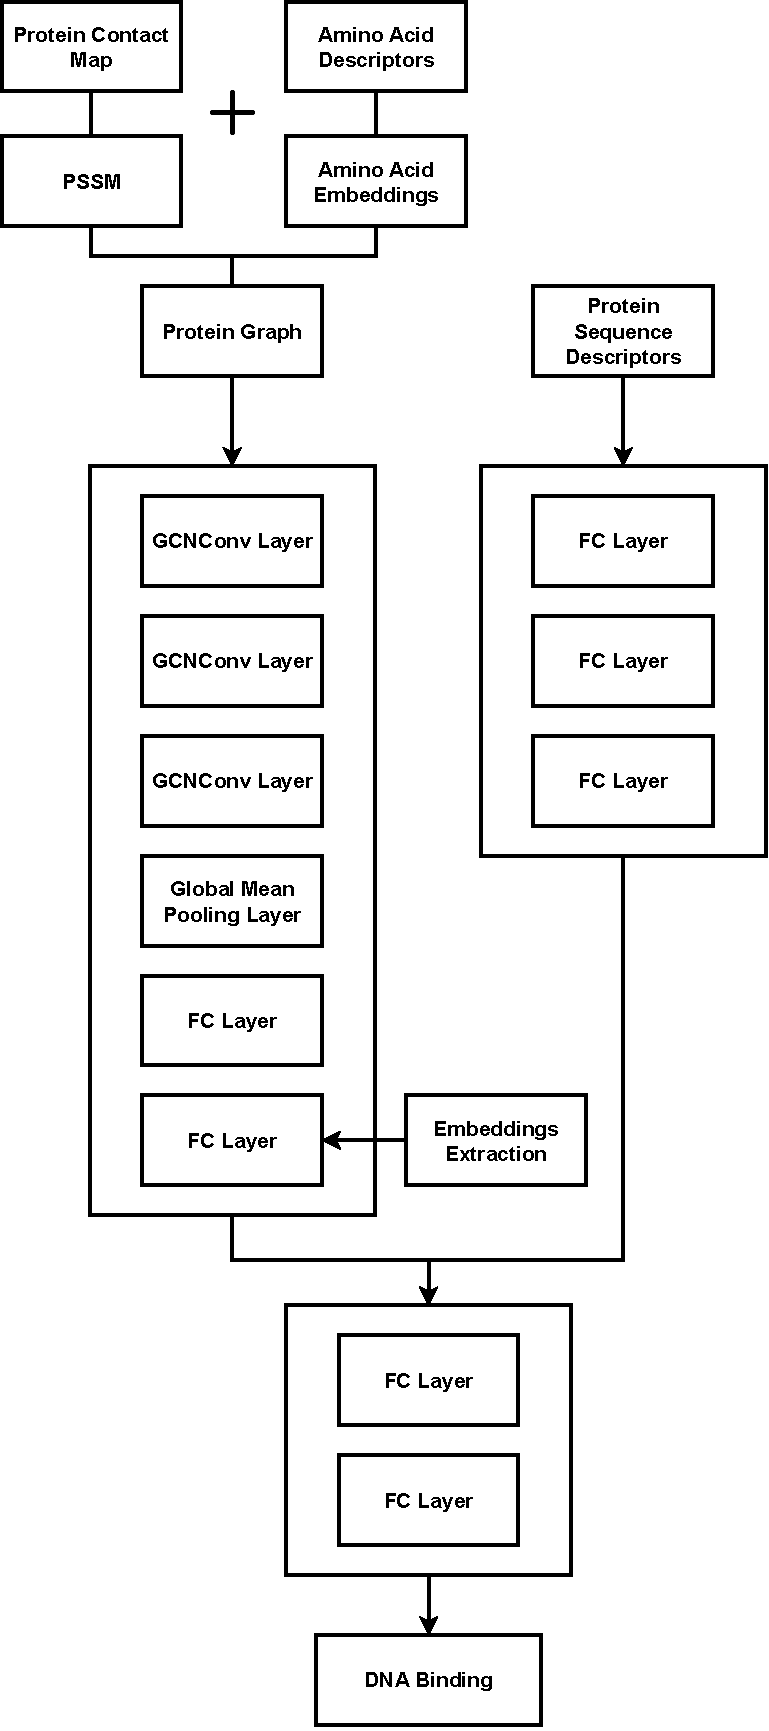
\includegraphics[width=1.0\linewidth]{images/Embeddings_NN_Architecture.pdf}    
    \caption{Figure showcasing our embedding model's architecture.}
    \label{fig:Embeddings_NN_Architecture} 
\end{figure}

\subsubsection{Embedding Extraction}
\label{subsubsec:Embedding_Extraction}

To extract our embeddings from our trained model we would use a forward hook on the second dense linear layer before the concatenation, showcased in Figure \ref{fig:Embeddings_NN_Architecture}, and perform a sequential forward pass over all of our proteins. Each forward pass would extract the embedding and place it into a dictionary which we would then use with our models.

\begin{figure*}[!h]
    \centering
    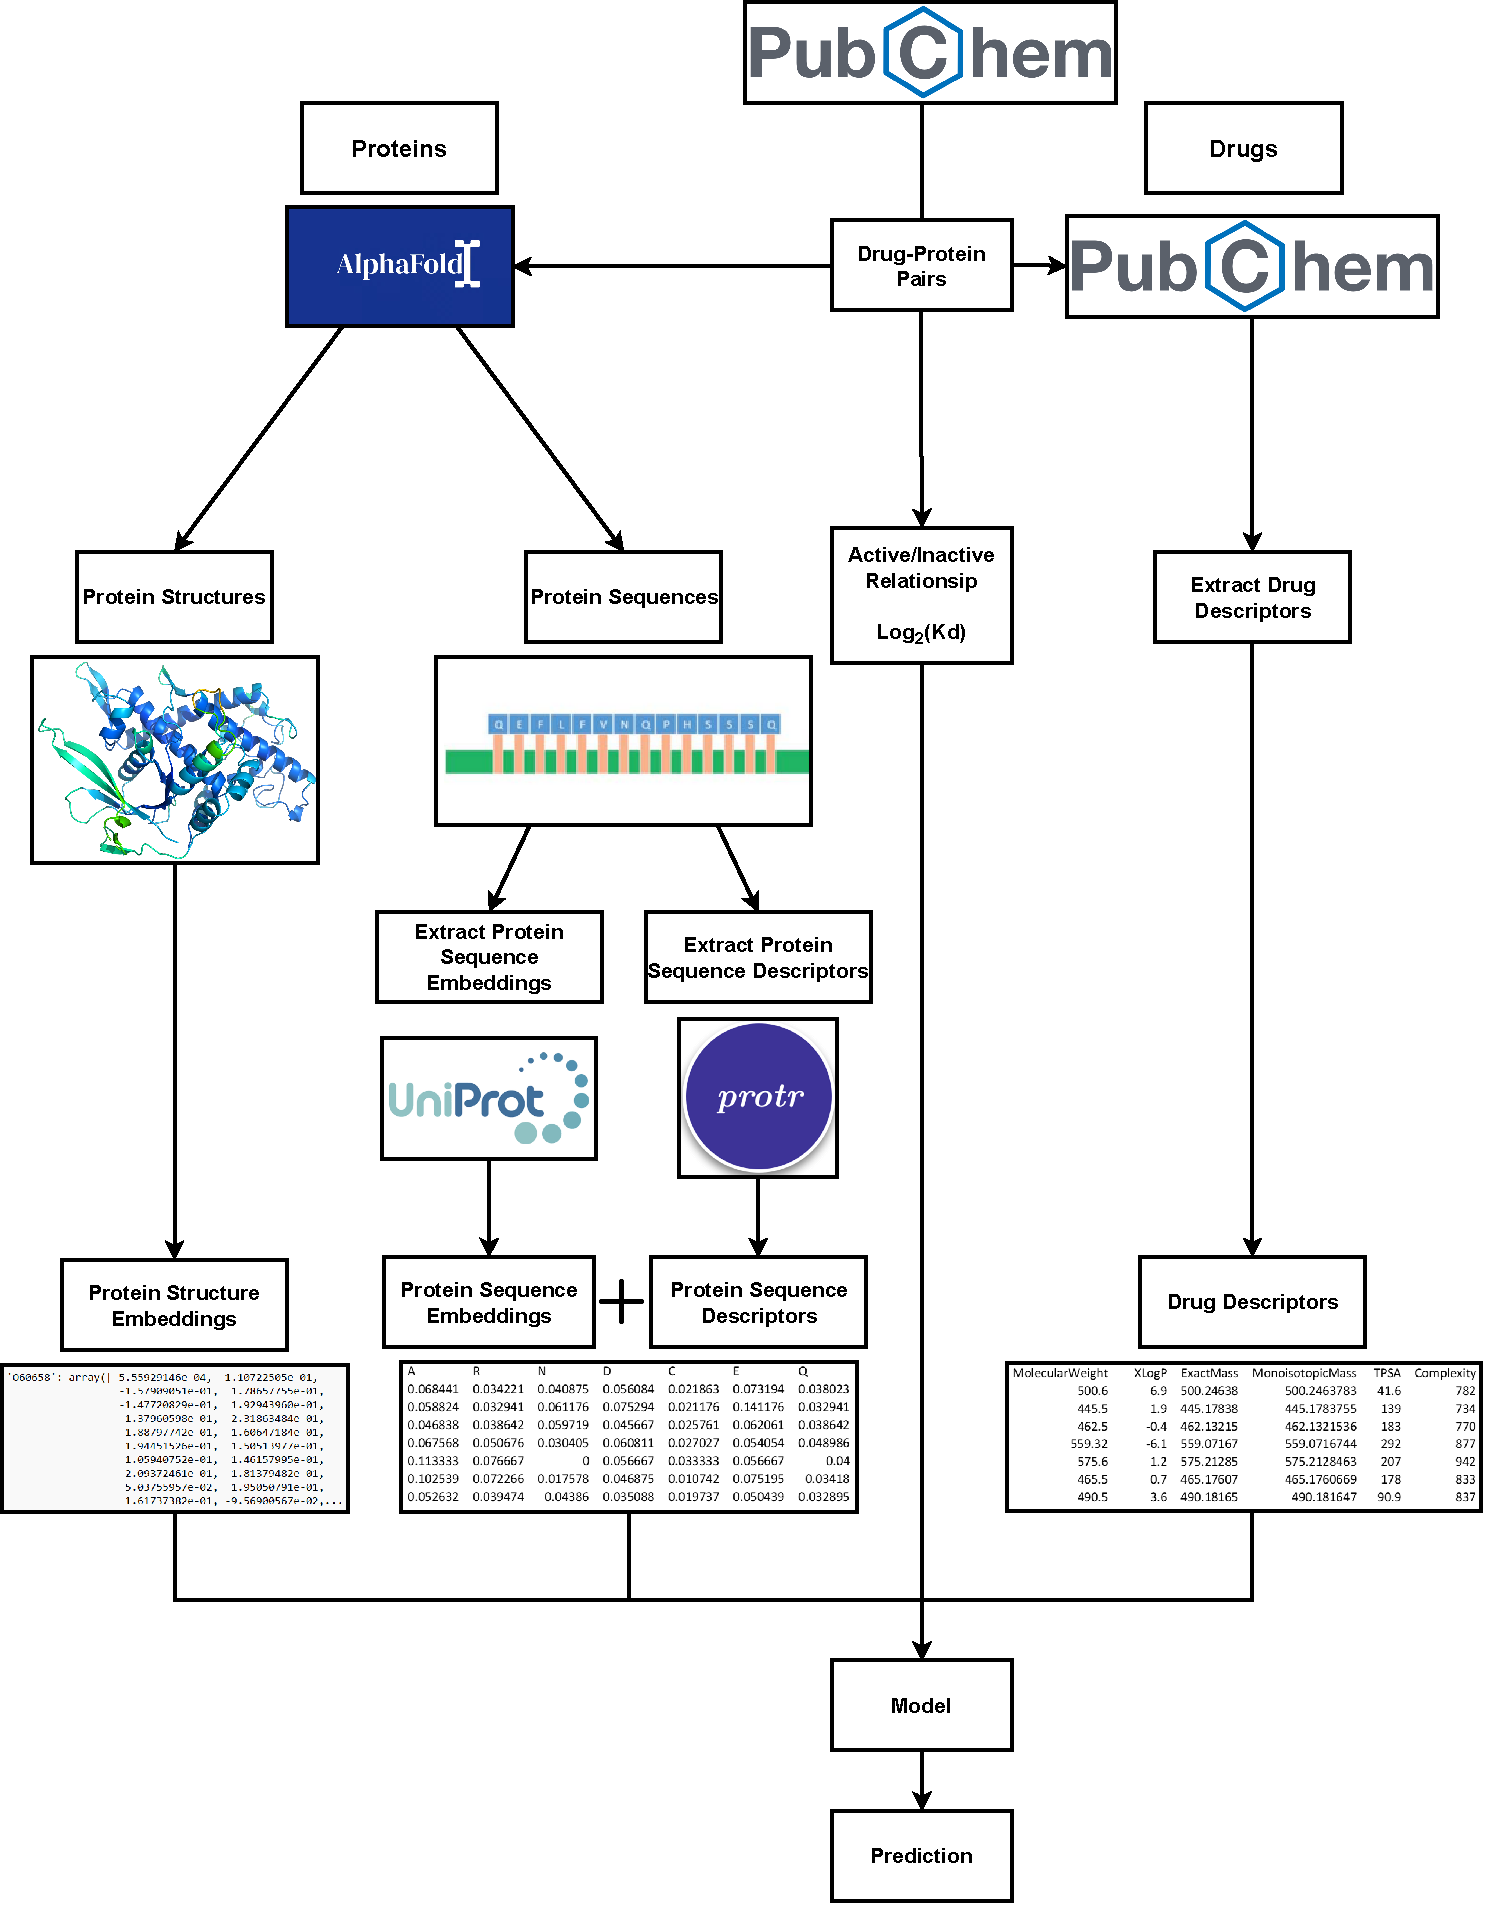
\includegraphics[width=0.95\linewidth]{images/DTIs_Methodology.pdf}    
    \caption{Figure showcasing our methodology behind the DTI models.}
    \label{fig:DTIs_Methodology} 
\end{figure*}

\begin{figure*}[!h]
    \centering
    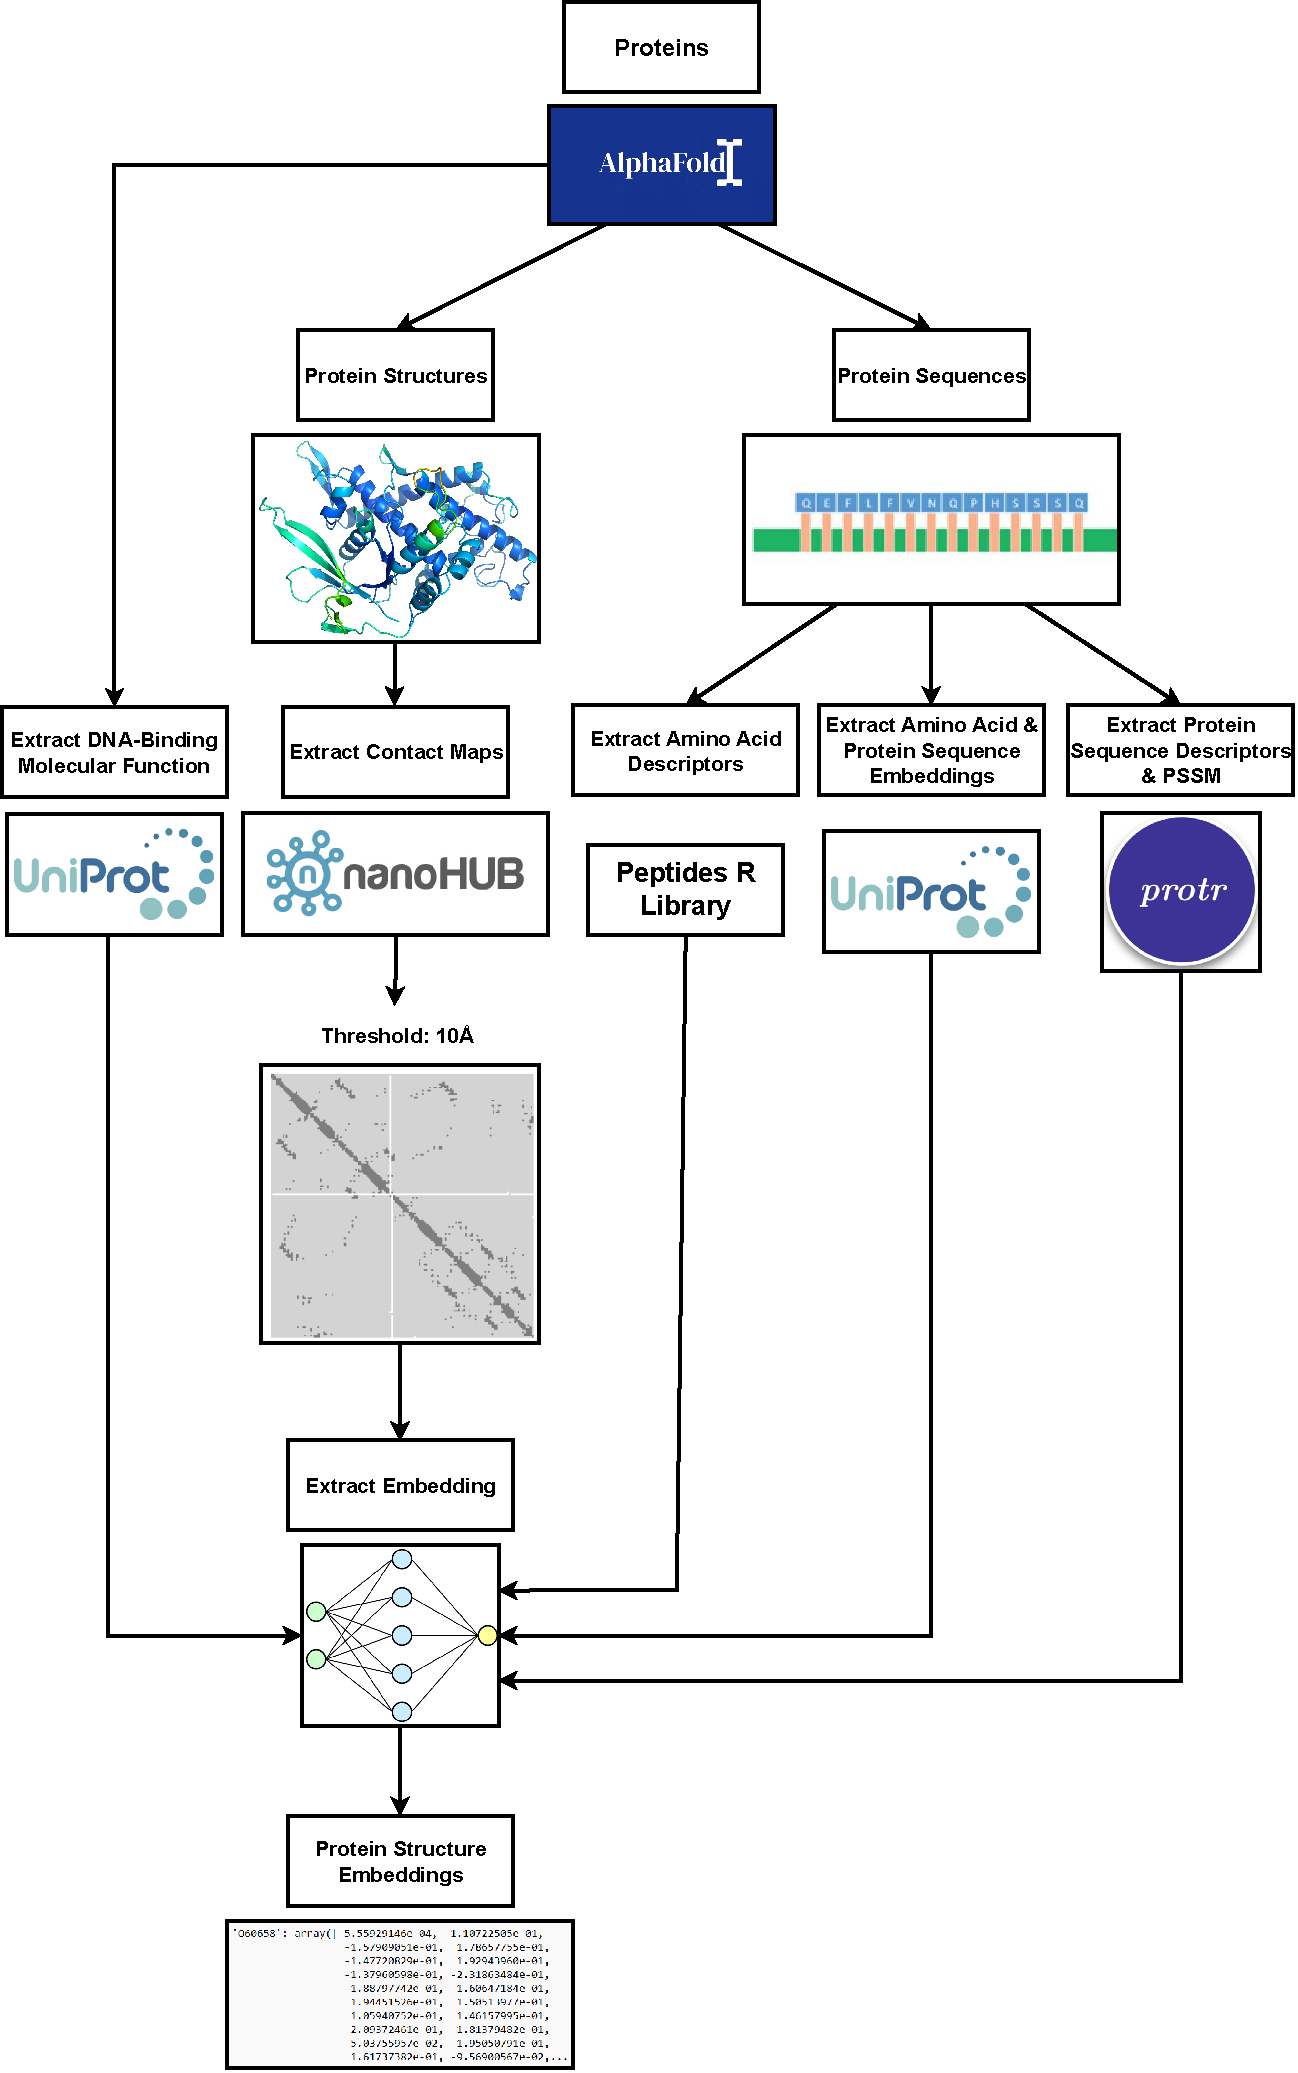
\includegraphics[width=0.78\linewidth]{images/Embeddings_Methodology.pdf}    
    \caption{Figure showcasing our methodology behind the embedding model.}
    \label{fig:Embeddings_Methodology} 
\end{figure*}


